%\usepackage[spanish]{babel}
\chapter{Introducción}

Esta salida corresponde al diseño especifico de pruebas. Estas son aisladas en \textbf{Escenarios de uso} a los que se acomplan una serie de \textbf{Casos de uso}. La ejecución es realizada por los encagardos de la validación en conformidad con las politicas de acceso, con especial énfasis en la aplicación de los protocolos que resguarden la integridad y persistencia de los datos.

\chapter{Nivel especifico de pruebas - Agilent OpenLAB}
\section{Nivel de pruebas - Funcionales}

\begin{figure}[H]
	\centering
	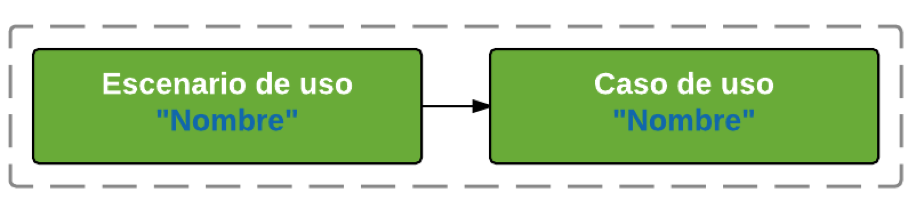
\includegraphics[width=0.7\linewidth]{img/pruebasfuncionales.png}
	\caption{Prueba funcional genérica}
	\label{fig:MarcoTeorico}
\end{figure}

\begin{table}[H]
	\begin{center}
		\begin{tabular}{|l|l|}
			\hline
			Escenario de prueba &  Caso de uso\\
			\hline \hline
			Parametros de entrada & \\ \hline
			Salida esperada & \\ \hline
			\hline \hline
			Resultado: & \\ \hline
			
		\end{tabular}
		\caption{Tabla de ejecución genérica}
		\label{tabla:sencilla}
	\end{center}
\end{table}

\newpage

\subsection{Pruebas CRUD método}

\subsubsection{Crear método}

\begin{figure}[H]
	\centering
	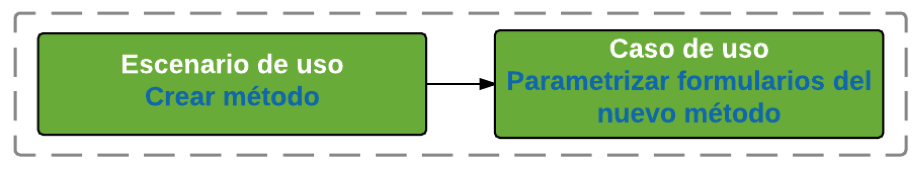
\includegraphics[width=0.7\linewidth]{img/crearmetodo.png}
	\caption{Prueba funcional crear}
	\label{fig:MarcoTeorico}
\end{figure}

\begin{table}[htbp]
	\begin{center}
		\begin{tabular}{|l|l|}
			\hline
			Crear método & Parametrizar formularios del nuevo método\\
			\hline \hline
			Parametros Column oven & Temperature, Stoptime, + - range \\ \hline
			Parametros Grad. Pump & Flow, Solvents \\ \hline
			Parametros DAD & Signals \\ \hline
			Parametros Sampler & Inyection volumen \\ \hline
			Salida esperada & Método creado con éxito\\ \hline
			\hline \hline
			Resultado: & \\ \hline
			
		\end{tabular}
		\caption{Tabla de ejecución crear método}
		\label{tabla:sencilla}
	\end{center}
\end{table}

\subsubsection{Leer método}

\begin{figure}[H]
	\centering
	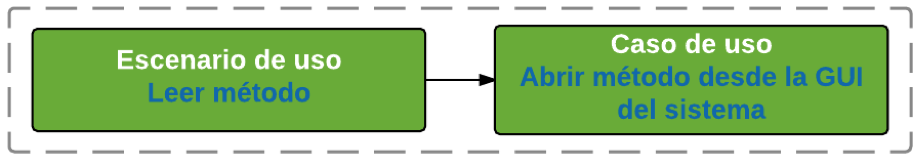
\includegraphics[width=0.7\linewidth]{img/leermetodo.png}
	\caption{Prueba funcional leer}
	\label{fig:MarcoTeorico}
\end{figure}

\begin{table}[H]
	\begin{center}
		\begin{tabular}{|l|l|}
			\hline
			Leer método & Abrir método desde la GUI del sistema \\
			\hline \hline
			Parametros de entrada & Método existente \\ \hline
			Salida esperada & Vista del método\\ \hline
			\hline \hline
			Resultado: & \\ \hline
			
		\end{tabular}
		\caption{Tabla de ejecución leer método}
		\label{tabla:sencilla}
	\end{center}
\end{table}


\subsubsection{Editar método}

\begin{figure}[H]
	\centering
	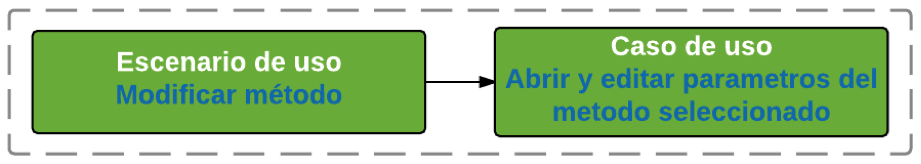
\includegraphics[width=0.7\linewidth]{img/modificarmetodo.png}
	\caption{Prueba funcional editar}
	\label{fig:MarcoTeorico}
\end{figure}

\begin{table}[H]
	\begin{center}
		\begin{tabular}{|l|l|}
			\hline
			Crear método & Abrir y editar parametros del método seleccionado \\
			\hline \hline
			Parametros Column oven & Temperature, Stoptime, + - range \\ \hline
			Parametros Grad. Pump & Flow, Solvents \\ \hline
			Parametros DAD & Signals \\ \hline
			Parametros Sampler & Inyection volumen \\ \hline
			Salida esperada & Nueva versión \\ \hline
			\hline \hline
			Resultado: & \\ \hline
			
		\end{tabular}
		\caption{Tabla de ejecución editar método}
		\label{tabla:sencilla}
	\end{center}
\end{table}


\subsubsection{Eliminar método}

\begin{figure}[H]
	\centering
	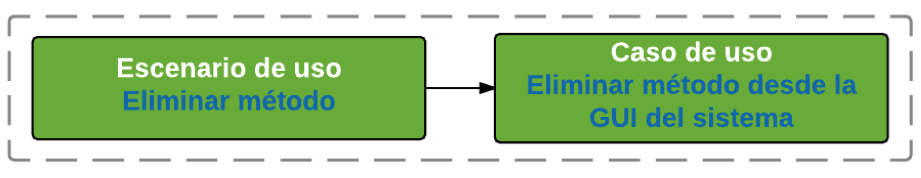
\includegraphics[width=0.7\linewidth]{img/eliminarmetodo.png}
	\caption{Prueba funcional eliminar}
	\label{fig:MarcoTeorico}
\end{figure}

\begin{table}[H]
	\begin{center}
		\begin{tabular}{|l|l|}
			\hline
			Eliminar método &  Eliminar método desde las GUI del sistema\\
			\hline \hline
			Parametros de entrada &  Método existente \\ \hline
			Salida esperada & Método eliminado \\ \hline
			\hline \hline
			Resultado: & \\ \hline
			
		\end{tabular}
		\caption{Tabla de ejecución eliminar método}
		\label{tabla:sencilla}
	\end{center}
\end{table}

\subsection{Pruebas CRUD secuencia}
\subsubsection{Crear secuencia}

\begin{figure}[H]
	\centering
	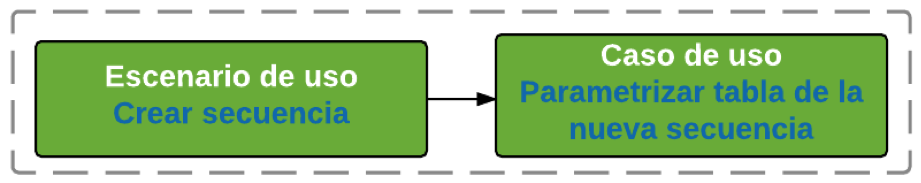
\includegraphics[width=0.7\linewidth]{img/crearsecuencia.png}
	\caption{Prueba funcional crear secuencia}
	\label{fig:MarcoTeorico}
\end{figure}

\begin{table}[htbp]
	\begin{center}
		\begin{tabular}{|l|l|}
			\hline
			Crear secuencia & Parametrizar tabla de la nueva secuencia\\
			\hline \hline
			Parametros de la secuencia & Run type, Custom, Reps, Vial, Volume, ID, Method, Name \\ \hline
			Parametros de secuencia (File name) & Data file \\ \hline
			Indicar salida & File paths Method, File paths Data \\ \hline
			Salida esperada & Secuencia creada con éxito \\ \hline
			\hline \hline
			Resultado: & \\ \hline	
		\end{tabular}
		\caption{Tabla de ejecución crear secuencia}
		\label{tabla:sencilla}
	\end{center}
\end{table}

\subsubsection{Leer secuencia}

\begin{figure}[H]
	\centering
	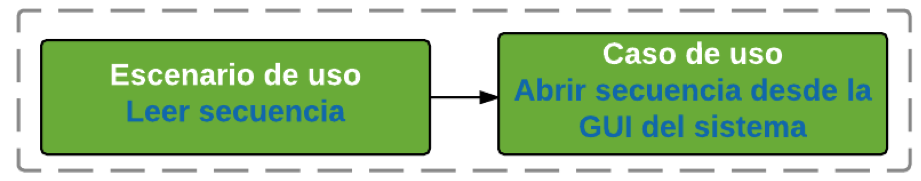
\includegraphics[width=0.7\linewidth]{img/leersecuencia.png}
	\caption{Prueba funcional leer secuencia}
	\label{fig:MarcoTeorico}
\end{figure}

\begin{table}[H]
	\begin{center}
		\begin{tabular}{|l|l|}
			\hline
			Leer secuencia & Abrir secuencia desde la GUI del sistema \\
			\hline \hline
			Parametros de entrada & Secuencia existente \\ \hline
			Salida esperada & Vista de la secuencia\\ \hline
			\hline \hline
			Resultado: & \\ \hline
			
		\end{tabular}
		\caption{Tabla de ejecución leer secuencia}
		\label{tabla:sencilla}
	\end{center}
\end{table}

\subsubsection{Editar secuencia}

\begin{figure}[H]
	\centering
	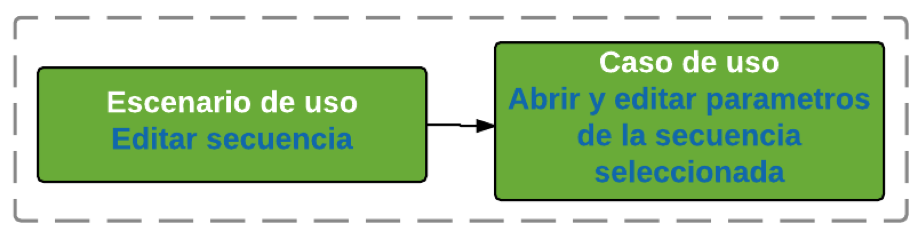
\includegraphics[width=0.7\linewidth]{img/editarsecuencia.png}
	\caption{Prueba funcional editar}
	\label{fig:MarcoTeorico}
\end{figure}

\begin{table}[H]
	\begin{center}
		\begin{tabular}{|l|l|}
			\hline
			Editar secuencia & Abrir y editar parametros de la secuencia seleccionada \\
			\hline \hline
		Parametros de la secuencia & Run type, Custom, Reps, Vial, Volume, ID, Method, Name \\ \hline
		Salida esperada & Nueva versión de la secuencia \\ \hline
		\hline \hline
		Resultado: & \\ \hline			
		\end{tabular}
		\caption{Tabla de ejecución editar secuencia}
		\label{tabla:sencilla}
	\end{center}
\end{table}

\subsubsection{Eliminar secuencia}

\begin{figure}[H]
	\centering
	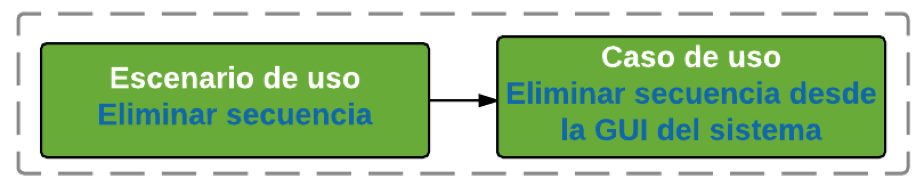
\includegraphics[width=0.7\linewidth]{img/eliminarsecuencia.png}
	\caption{Prueba funcional eliminar secuencia}
	\label{fig:MarcoTeorico}
\end{figure}

\begin{table}[H]
	\begin{center}
		\begin{tabular}{|l|l|}
			\hline
			Eliminar método &  Eliminar secuencia desde la GUI del sistema\\
			\hline \hline
			Parametros de entrada &  Secuencia existente \\ \hline
			Salida esperada & Secuencia eliminada \\ \hline
			\hline \hline
			Resultado: & \\ \hline
		\end{tabular}
		\caption{Tabla de ejecución eliminar secuencia}
		\label{tabla:sencilla}
	\end{center}
\end{table}

\subsubsection{Reprocesar secuencia}
\begin{figure}[H]
	\centering
	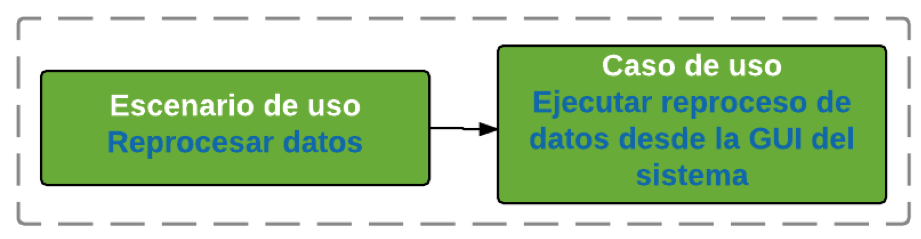
\includegraphics[width=0.7\linewidth]{img/reprocesar.png}
	\caption{Prueba funcional reprocesar secuencia}
	\label{fig:MarcoTeorico}
\end{figure}
\begin{table}[H]
	\begin{center}
		\begin{tabular}{|l|l|}
			\hline
			Reprocesar datos &  Ejecutar reproceso de datos desde la GUI del sistema\\
			\hline \hline
			Parametros de entrada & Método, Secuencia, Inyección, Limites de integración/retención \\ \hline
			Salida esperada & Reporte\\ \hline
			\hline \hline
			Resultado: & \\ \hline
		\end{tabular}
		\caption{Tabla de ejecución reproceso de datos}
		\label{tabla:sencilla}
	\end{center}
\end{table}

\chapter{Nivel especifico de pruebas - TotalChrom}

\section{Nivel de pruebas - Funcionales}
\subsection{Pruebas CRUD método}
\subsubsection{Crear método}

\begin{figure}[H]
	\centering
	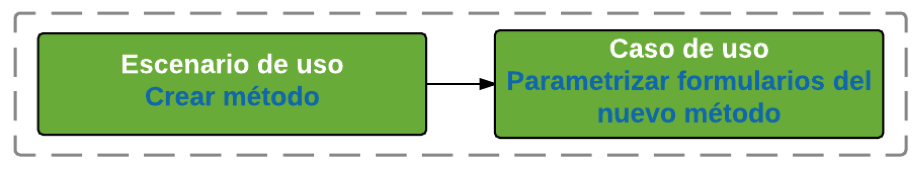
\includegraphics[width=0.7\linewidth]{img/crearmetodo.png}
	\caption{Prueba funcional crear}
	\label{fig:MarcoTeorico}
\end{figure}

\begin{table}[htbp]
	\begin{center}
		\begin{tabular}{|l|l|}
			\hline
			Crear método & Parametrizar formularios \\
			\hline \hline
			Parametros Autosampler & Preinjection, Solvent washes \\ \hline
			Parametros Oven ramp & Rate, temp, hold \\ \hline
			Parametros Carrier & Rate, Setpoint, Hold, Lenght, Diameter \\ \hline
			Parametros Detectors  & Temperature, range \\ \hline
			Parametros Instrument time events  &  Time, Event, Value \\ \hline
			Salida esperada & Método creado con éxito\\ \hline
			\hline \hline
			Resultado: & \\ \hline
			
		\end{tabular}
		\caption{Tabla de ejecución crear método}
		\label{tabla:sencilla}
	\end{center}
\end{table}

\subsubsection{Leer método}

\begin{figure}[H]
	\centering
	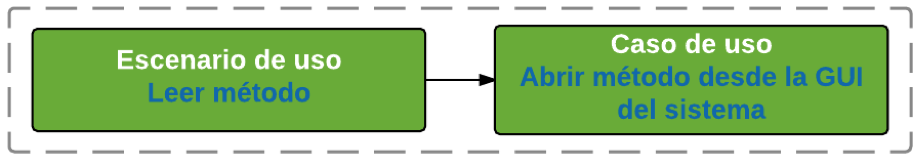
\includegraphics[width=0.7\linewidth]{img/leermetodo.png}
	\caption{Prueba funcional leer}
	\label{fig:MarcoTeorico}
\end{figure}

\begin{table}[H]
	\begin{center}
		\begin{tabular}{|l|l|}
			\hline
			Leer método & Método existente \\
			\hline \hline
			Parametros de entrada & Método existente \\ \hline
			Salida esperada & Vista del método\\ \hline
			\hline \hline
			Resultado: & \\ \hline
			
		\end{tabular}
		\caption{Tabla de ejecución leer método}
		\label{tabla:sencilla}
	\end{center}
\end{table}


\subsubsection{Editar método}

\begin{figure}[H]
	\centering
	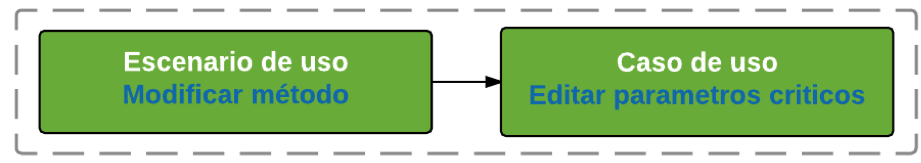
\includegraphics[width=0.7\linewidth]{img/editarmetodo.png}
	\caption{Prueba funcional editar}
	\label{fig:MarcoTeorico}
\end{figure}

\begin{table}[H]
	\begin{center}
		\begin{tabular}{|l|l|}
			\hline
		Editar método & Parametrizar formularios \\
		\hline \hline
		Parametros Autosampler & Preinjection, Solvent washes \\ \hline
		Parametros Oven ramp & Rate, temp, hold \\ \hline
		Parametros Carrier & Rate, Setpoint, Hold, Lenght, Diameter \\ \hline
		Parametros Detectors  & Temperature, range \\ \hline
		Parametros Instrument time events  &  Time, Event, Value \\ \hline
		Salida esperada & Nueva versión del método\\ \hline
		\hline \hline
		Resultado: & \\ \hline
		
			
		\end{tabular}
		\caption{Tabla de ejecución editar método}
		\label{tabla:sencilla}
	\end{center}
\end{table}


\subsubsection{Eliminar método}

\begin{figure}[H]
	\centering
	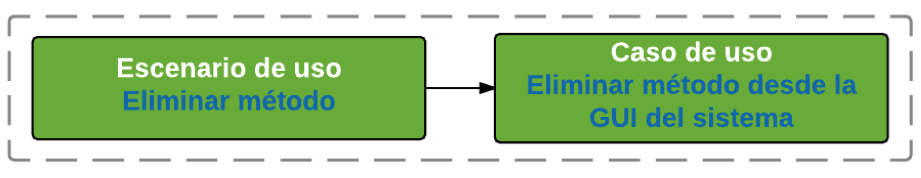
\includegraphics[width=0.7\linewidth]{img/eliminarmetodo.png}
	\caption{Prueba funcional eliminar}
	\label{fig:MarcoTeorico}
\end{figure}

\begin{table}[H]
	\begin{center}
		\begin{tabular}{|l|l|}
			\hline
			Eliminar método &  Seleccionar el método a eliminar\\
			\hline \hline
			Parametros de entrada &  Método existente \\ \hline
			Salida esperada & Método eliminado \\ \hline
			\hline \hline
			Resultado: & \\ \hline
			
		\end{tabular}
		\caption{Tabla de ejecución eliminar método}
		\label{tabla:sencilla}
	\end{center}
\end{table}

\subsection{Pruebas CRUD secuencia}
\subsubsection{Crear secuencia}

\begin{figure}[H]
	\centering
	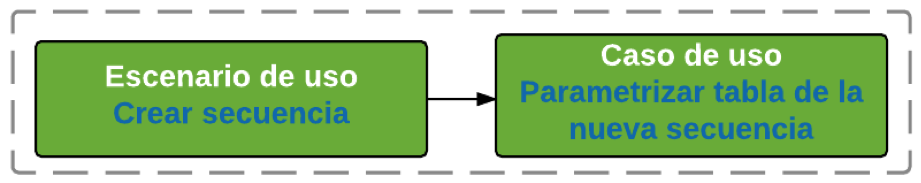
\includegraphics[width=0.7\linewidth]{img/crearsecuencia.png}
	\caption{Prueba funcional crear secuencia}
	\label{fig:MarcoTeorico}
\end{figure}

\begin{table}[htbp]
	\begin{center}
		\begin{tabular}{|l|l|}
			\hline
			Crear secuencia & Parametrizar tabla \\
			\hline \hline
			Parametros de la secuencia & Type, Name, Number, Method, Vial, ID\\ \hline
			Indicar rutas & File paths Method, File paths Data \\ \hline
			Salida esperada & Secuencia creada \\ \hline
			\hline \hline
			Resultado: & \\ \hline	
		\end{tabular}
		\caption{Tabla de ejecución crear secuencia}
		\label{tabla:sencilla}
	\end{center}
\end{table}

\subsubsection{Leer secuencia}

\begin{figure}[H]
	\centering
	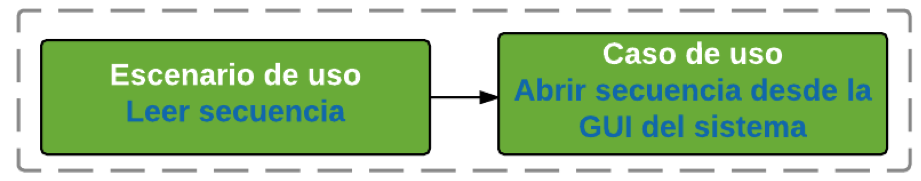
\includegraphics[width=0.7\linewidth]{img/leersecuencia.png}
	\caption{Prueba funcional leer secuencia}
	\label{fig:MarcoTeorico}
\end{figure}

\begin{table}[H]
	\begin{center}
		\begin{tabular}{|l|l|}
			\hline
			Leer secuencia & Abrir secuencia \\
			\hline \hline
			Parametros de entrada & Secuencia existente \\ \hline
			Salida esperada & Vista de la secuencia\\ \hline
			\hline \hline
			Resultado: & \\ \hline
			
		\end{tabular}
		\caption{Tabla de ejecución leer secuencia}
		\label{tabla:sencilla}
	\end{center}
\end{table}

\subsubsection{Editar secuencia}

\begin{figure}[H]
	\centering
	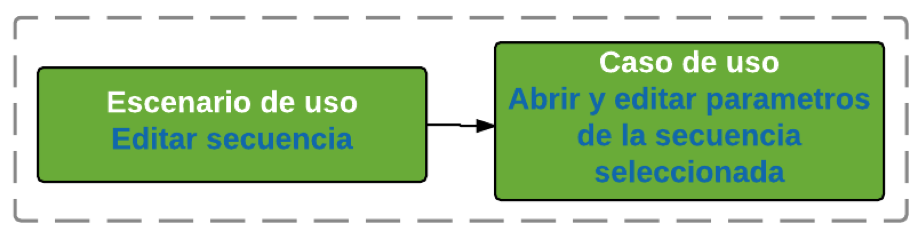
\includegraphics[width=0.7\linewidth]{img/editarsecuencia.png}
	\caption{Prueba funcional editar}
	\label{fig:MarcoTeorico}
\end{figure}

\begin{table}[H]
	\begin{center}
		\begin{tabular}{|l|l|}
			\hline
			Editar secuencia & Modificar Parametros \\
			\hline \hline
			Parametros de la secuencia & Type, Name, Number, Method, Vial, ID\\ \hline
			Indicar rutas & File paths Method, File paths Data \\ \hline
			Salida esperada & Nueva versión de la secuencia \\ \hline
			\hline \hline
			Resultado: & \\ \hline			
		\end{tabular}
		\caption{Tabla de ejecución editar secuencia}
		\label{tabla:sencilla}
	\end{center}
\end{table}

\subsubsection{Eliminar secuencia}

\begin{figure}[H]
	\centering
	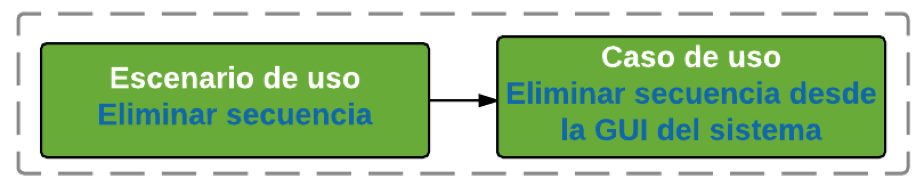
\includegraphics[width=0.7\linewidth]{img/eliminarsecuencia.png}
	\caption{Prueba funcional eliminar secuencia}
	\label{fig:MarcoTeorico}
\end{figure}

\begin{table}[H]
	\begin{center}
		\begin{tabular}{|l|l|}
			\hline
			Eliminar método &  Seleccionar secuencia\\
			\hline \hline
			Parametros de entrada &  Secuencia existente \\ \hline
			Salida esperada & Secuencia eliminada \\ \hline
			\hline \hline
			Resultado: & \\ \hline
		\end{tabular}
		\caption{Tabla de ejecución eliminar secuencia}
		\label{tabla:sencilla}
	\end{center}
\end{table}

\subsubsection{Reprocesar secuencia}
\begin{figure}[H]
	\centering
	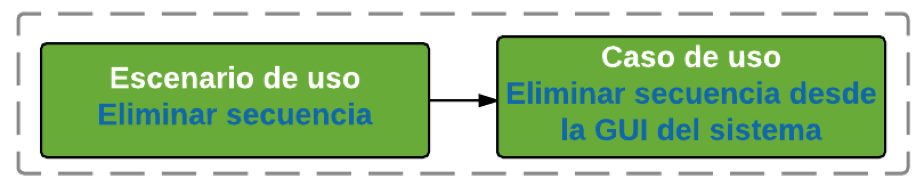
\includegraphics[width=0.7\linewidth]{img/eliminarsecuencia.png}
	\caption{Prueba funcional reprocesar}
	\label{fig:MarcoTeorico}
\end{figure}
\begin{table}[H]
	\begin{center}
		\begin{tabular}{|l|l|}
			\hline
			Eliminar método &  Seleccionar secuencia\\
			\hline \hline
			Parametros de entrada & Secuencia, Limites de integración/retención \\ \hline
			Salida esperada & Reporte \\ \hline
			\hline \hline
			Resultado: & \\ \hline
		\end{tabular}
		\caption{Tabla de ejecución reprocesar}
		\label{tabla:sencilla}
	\end{center}
\end{table}

\chapter{Nivel especifico de pruebas - Bettersize}
\section{Nivel de pruebas - Funcionales}
\subsubsection{Test document}

\begin{figure}[H]
	\centering
	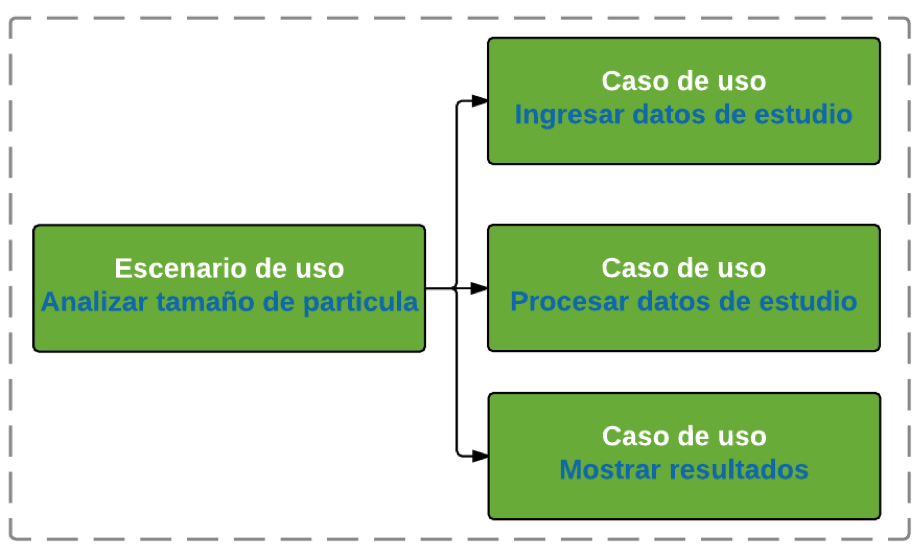
\includegraphics[width=0.6\linewidth]{img/bettersize.png}
	\caption{Prueba funcional ingresar datos}
	\label{fig:MarcoTeorico}
\end{figure}

\begin{table}[H]
	\begin{center}
		\begin{tabular}{|l|l|}
		\hline
		Analizar tamaño de particula & Ingresar datos de estudio\\
		\hline \hline
		Parametros de entrada & Sample name, Medium name, Operator, Date, Time \\ \hline
		Parametros de entrada & MeasureDept, SampleOwner, Remark \\ \hline
		Salida esperada & Datos ingresados \\ \hline
		\hline \hline
		Resultado: & \\ \hline
		\end{tabular}
		\caption{Tabla de ejecución ingresar datos}
		\label{tabla:sencilla}
	\end{center}
\end{table}

\begin{table}[H]
	\begin{center}
		\begin{tabular}{|l|l|}
		      \hline
		Analizar tamaño de particula & Procesar datos de estudio\\
		\hline \hline
		Parametros de entrada & Sample result  \\ \hline
		Salida esperada & Datos procesados \\ \hline
		\hline \hline
		Resultado: & \\ \hline
		\end{tabular}
		\caption{Tabla de ejecución procesar datos}
		\label{tabla:sencilla}
	\end{center}
\end{table}


\begin{table}[H]
	\begin{center}
		\begin{tabular}{|l|l|}
		  \hline
		Analizar tamaño de particula & Mostrar resultados\\
		\hline \hline
		Parametros de entrada & Submit Preview\\ \hline
		Salida esperada & Vista de los resultados\\ \hline
		\hline \hline
		Resultado: & \\ \hline
		\end{tabular}
		\caption{Tabla de ejecución mostrar resultados}
		\label{tabla:sencilla}
	\end{center}
\end{table}


